\subsection{大容量强磁吸附工具结构及工作原理}
大容量强磁吸附工具\footnote{下文简称“强磁工具”}用于打捞石油、地质钻、修套管清洁作业过程中产生的不能被循环液返出的磁性碎物，通过永久磁铁吸附磁性碎物并将其带出井筒，实现井筒净化效果。针对不同尺寸磁性碎物，磁铁套筒有两种吸附模式，一种是沿侧面沟槽方向吸附，另一种是沿圆周方向吸附，两种强磁均具有保护层，可单独更换强磁块，且强磁块固定未采用螺钉连接，方便装卸且结构稳定。针对套管中磁性碎物的含量，可以预先装配不同数量的磁铁套筒，以匹配强磁吸附工具容量和磁性碎物量。该工具具有结构可靠、操作方便、多方向，多尺寸吸附、碎屑吸附量大和可调节等优点。

强磁工具主要由上接头、上连接套、侧吸强磁部件、中间连接套、环吸强磁部件、止退环、下接头等零件组成。
通过永久磁铁吸附磁性碎物并将其带出井筒，从井下回收不能被循环液返出的磁性碎物，从而实现井筒净化效果。


\begin{table}[htbp]
    \centering
    \caption{强磁工具技术参数}
    \label{tab:dqc_parameters}
    \renewcommand{\arraystretch}{1.3} % 增加行高，使表格不拥挤
    \small % 如果表格太宽，可以使用 \small 或 \footnotesize 微调字号
    
    % 使用 tabularx 环境，总宽度设为 \textwidth
    % 列定义说明：
    % l: 左对齐（型号）
    % c: 居中对齐（数值类数据）
    % X: 自动伸缩列（用于较长文本或为了撑满宽度的列，这里用于平衡布局）
    \begin{tabularx}{.9\textwidth}{l ccc Xc ccc c} 
        \toprule
        % 表头内容
        规格 & 
        \begin{tabular}[c]{@{}c@{}}接头\\外径\\ (mm)\end{tabular} & 
        \begin{tabular}[c]{@{}c@{}}扶正\\外径\\ (mm)\end{tabular} & 
        \begin{tabular}[c]{@{}c@{}}本体\\外径\\ (mm)\end{tabular} & 
        \begin{tabular}[c]{@{}c@{}}适用套\\管磅级\\ (lb/ft)\end{tabular} & 
        \begin{tabular}[c]{@{}c@{}}水眼\\ (mm)\end{tabular} & 
        \begin{tabular}[c]{@{}c@{}}总长\\ (mm)\end{tabular} & 
        \begin{tabular}[c]{@{}c@{}}接头\\螺纹\\ (API)\end{tabular} & 
        \begin{tabular}[c]{@{}c@{}}抗拉\\强度\\ (kN)\end{tabular} & 
        \begin{tabular}[c]{@{}c@{}}抗扭\\强度\\ (kN$\cdot$m)\end{tabular} \\
        \midrule
        
        % 数据行
        7\inch  & 127    & 141.5  & 139.7  & 9.5-40.5 & 40    & 6500 & NC38      & 1800 & 21  \\
        9-5/8\inch  & 165    & 185.93 & 184.15 & ALL      & 57.15 & 6500 & NC50      & 3500 & 30  \\
        13-3/8\inch  & 196    & 236.73 & 234.95 & ALL      & 76.2  & 6500 & 6 5/8 REG & 5000 & 60  \\
        
        \bottomrule
    \end{tabularx}
\end{table}
%[c]{@{}c@{}}中方括号内的 [c] 是垂直对齐参数，用于控制该 tabular 环境作为一个整体在其所在行中的垂直位置。@{}c@{} 是表格列格式定义，其核心作用是控制单元格内容的对齐方式并消除列间默认间距，常用于嵌套表格或需要精确对齐的场景
%lb/ft为“磅每英尺”，lb 是英制质量单位磅（Pound）的缩写，英语中的 "pound" 一词本身就源自拉丁语 pondus（重量），因此保留了 libra 的缩写 lb 作为符号

\subsection{强磁工具结构设计}

这里缺内容

\subsection[强磁工具结构设计计算与校核]{强磁工具结构设计计算与校核\protect\footnote{合同条款：5.2.1.3井筒高效清洁关键技术配套工具设计——（2）大容量强磁吸附工具：抗拉$>=100T$，抗扭$>=18kN\cdot m$，吸附力$>=8kg/cm^2$，吸附容量$>=50L$}}

%这里的强度校核与四合一工具的相同，我这里姑且写上，后面可以引用前面的内容并把这个注释掉。

大容量强磁工具的主要受力件为芯轴，其连接螺纹为 2.85\inch-8 Stub ACME。螺纹牙剪切强度计算：

\begin{align}
    F_{\max} &= [\tau] \cdot k_z \cdot \pi \cdot d_1 \cdot b \cdot z \times 10^{-3} \\
    [\tau] &= \frac{\sigma_s}{n}
\end{align}
式中，$F_{\max}$——工具最大拉力，kN；

$[\tau]$——螺纹牙的剪切强度，MPa；

$k_z$——螺纹各圈的载荷不均系数，根据《机械设计手册》，取 $k_z = 0.56$；

$d_1$——螺纹底径，mm；

$b$——螺纹牙根宽度，mm；

$n$——安全系数根据《机械设计手册》，取 $n = 2.5$；

$z$——旋合圈数；

$\sigma_s$——材料最小屈服强度：930 MPa (4330V-155KSI)。


2.85\inch-8 Stub ACME 螺纹代入数据计算如下：
\begin{align}
    F_{\max} &= [\tau] \cdot k_z \cdot \pi \cdot d_1 \cdot b \cdot z \times 10^{-3} \\
             &= 372 \times 0.56 \times 3.14 \times 70.30 \times 1.833 \times 35 \times 10^{-3} \\
             &= 2950.16 \, \text{kN} \\
             &> 1000 \, \text{kN}
\end{align}

于是，螺纹的强度满足设计要求。

大容量强磁工具的主要受力件为芯轴,危险截面有两处，分别为2.85\inch -8 Stub ACME外螺纹根部、2.85\inch-8 Stub ACME内螺纹根部。下面为芯轴抗拉计算：
%这里的2.85是不是写错了

（1）轴抗拉危险截面1：为2.85\inch -8 Stub ACME外螺纹根部

抗拉强度$F_{\max}$为
\begin{align}
    F_{\max} &= \left[\pi \cdot (D^2 - d^2)\right] \cdot \sigma_s / (4 \cdot n) \times 10^{-3}
\end{align}
式中，$F_{\max}$---工具最大拉力，kN；\\
$D$---危险截面外径，mm；\\
$d$---危险截面内径，mm；\\
$\sigma_s$---材料最小屈服强度：930 MPa (4330V-155KSI)；\\
$n$---安全系数，取 $n = 1.5$。

芯轴2.85\inch-8 Stub ACME 外螺纹根部最大拉力：
\begin{align}
    F_{\max} &= \left[\pi \cdot (D^2 - d^2) \cdot \sigma_s / (4 \cdot n)\right] \times 10^{-3} \\
             &= \left[3.14 \times (69.48^2 - 40^2) \times 930 / (4 \times 1.5)\right] \times 10^{-3} \\
             &= 1570.81 \, \text{kN} > 1000 \, \text{kN}
\end{align}
于是，外螺纹根部满足设计要求。

（2）芯轴抗拉危险截面2：为2.85\inch -8 Stub ACME内螺纹根部。

抗拉强度计算
\begin{equation}
    F_{\max} = \frac{[\pi \cdot (D^2 - d^2)] \cdot \sigma_s}{4 \cdot n} \times 10^{-3}
\end{equation}
式中，$F_{\max}$---工具最大拉力，kN；

$D$---危险截面外径，mm；

$d$---危险截面内径，mm；

$\sigma_s$---材料最小屈服强度：930MPa(4330V-155KSI)；

$n$---安全系数，取 $n = 1.5$。

芯轴 2.85\inch -8 Stub ACME 内螺纹根部最大拉力
\begin{align}
    F_{\max} &= \frac{\pi \cdot (D^2 - d^2) \cdot \sigma_s}{4 \cdot n} \times 10^{-3} \\
             &= \frac{3.14 \times (100^2 - 73^2) \times 930}{4 \times 1.5} \times 10^{-3} \\
             &= 2273.38 \text{kN} > 1000 \text{kN}
\end{align}

于是，内螺纹根部强度满足设计要求。


强磁工具在扭矩作用下，芯轴为危险零件,其危险截面有两处，分别为2.85\inch-8 Stub ACME外螺纹根部、2.85\inch -8 Stub ACME内螺纹根部。

(1)	芯轴抗扭危险截面1：为2.85”-8 Stub ACME外螺纹根部。

抗扭强度 $\tau$ 计算：
\begin{equation}
\begin{aligned}
    \tau &= \frac{16 \cdot D \cdot T_{\max}}{\pi \cdot (D^4 - d^4)} \times 10^6 \\
    T_{\max} &= \frac{[\tau] \cdot \pi \cdot (D^4 - d^4)}{16 \cdot D} \times 10^{-6}
    [\tau] &= n \cdot \sigma_s = 0.66 \times 930\,\text{MPa} = 613.8\,\text{MPa}
\end{aligned}
\end{equation}
式中，$T_{\max}$---最大扭矩，kN$\cdot$m；

$D$---危险截面外径，mm；

$d$---危险截面内径，mm；

$\sigma_s$---材料屈服应力，MPa；

$n$---许用剪应力与许用拉应力系数，根据《机械设计手册》，取 $n = 0.66$；

$[\tau]$---材料许用切应力，MPa。

芯轴 2.85\inch -8 Stub ACME 外螺纹根部最大扭矩：
\begin{align}
    T_{\max} &= \frac{[\tau] \cdot \pi \cdot (D^4 - d^4)}{16 \cdot D} \times 10^{-6} \\
             &= \frac{613.8 \times 3.14 \times (69.48^4 - 40^4)}{16 \times 69.48} \times 10^{-6} \\
             &= 35.96\,\text{kN}\cdot\text{m} > 18\,\text{kN}\cdot\text{m}
\end{align}

于是，心轴外螺纹根部抗扭强度满足设计要求。

（2）芯轴抗扭危险截面2：为2.85\inch -8 Stub ACME内螺纹根部。

抗扭强度 $\tau$ 计算：
\begin{align}
    \tau &= \frac{16 \cdot D \cdot T_{\max}}{\pi \cdot (D^4 - d^4)} \times 10^6 \\
    T_{\max} &= \frac{[\tau] \cdot \pi \cdot (D^4 - d^4)}{16 \cdot D} \times 10^{-6} \\
    [\tau] &= n \cdot \sigma_s = 0.66 \times 930\,\text{MPa} = 613.8\,\text{MPa}
\end{align}
式中，$T_{\max}$---工具最大扭矩，$\text{kN}\cdot\text{m}$；

$\sigma_s$---材料屈服应力，$\text{MPa}$；

$D$---危险截面外径，$\text{mm}$；

$d$---危险截面内径，$\text{mm}$；

$n$---许用剪应力与许用拉应力系数，根据《机械设计手册》，取 $n = 0.66$；

$[\tau]$---材料许用切应力，$\text{MPa}$。

芯轴 2.85\inch -8 Stub ACME 内螺纹根部最大扭矩：
\begin{align}
    T_{\max} &= \frac{[\tau] \cdot \pi \cdot (D^4 - d^4)}{16 \cdot D} \times 10^{-6} \\
             &= \frac{613.8 \times 3.14 \times (100^4 - 73^4)}{16 \times 100} \times 10^{-6} \\
             &= 86.25\,\text{kN}\cdot\text{m} > 18\,\text{kN}\cdot\text{m}
\end{align}

于是，内螺纹根部抗扭强度满足设计要求。

主要受力件为下接头，采用有限元方法进行计算，计算结果如图\ref{fig:torsion_stress_lowwer_sub_mag_tool}所示。危险截面出现在防退扣根部，最大剪切力为1030MPa，略高于屈服强度，属于应力集中导致的局部小尺度高应力，不会引发整体塑性变形，强度满足设计要求。
%这个说法是错误的
\begin{figure}[htbp]
    \centering
    % 子图 (a)
    \subfloat[大容量强磁工具下接头]{%
        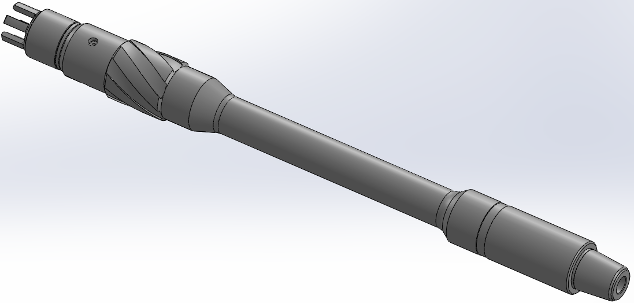
\includegraphics[width=0.5\linewidth]{figure/chapter3/lowwer-sub-mag-tool.png}%
        \label{fig:lowwer_sub_mag_tool}
    }
    \hfill
    % 子图 (b)
    \subfloat[受力件抗扭强度校核]{%
        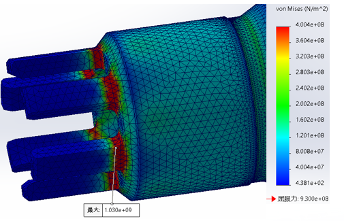
\includegraphics[width=0.4\linewidth]{figure/chapter3/torsion-stress-lowwer-sub-mag-tool.png}%
        \label{fig:torsion_stress_lowwer_sub_mag_tool.png}%
    }
        \caption{受力件抗扭强度有限元分析结果}
    \label{fig:torsion_stress_lowwer_sub_mag_tool}
\end{figure}






\subsubsection{吸附容量计算}

大容量强磁工具的吸附位置主要为四个强磁架处，上端两个强磁架相同，下端两个强磁架相同。
下面为大容量强磁工具吸附容量计算：

7\inch、17lb/ft套管，壁厚为5.87mm，内径为166.06mm。

吸附容量计算 $V_{\max}$ 计算：
\begin{equation}
    V_{\max} = (2 \cdot 5 \cdot s \cdot h + s_1 \cdot h_1 + s_2 \cdot h_2) \times 10^{-6}
\end{equation}
式中，$V_{\max}$---最大吸附容量，L；

$s$---上部强磁沟槽截面面积，$\text{mm}^2$；

$s_1$---上部强磁环空面积，$\text{mm}^2$；

$s_2$---下部强磁环空面积，$\text{mm}^2$；

$h$---强磁环长度，mm；

$h_1$---上部强磁环空长度，mm；

$h_1$---下部强磁环空长度，mm。

大容量强磁吸附容量：
\begin{equation}
	\begin{aligned}
    V_{\max} &= (2 \times 5 \times 603 \times 500 + 7340 \times 1438 + 10343 \times 1420) \times 10^{-6} \\
             &= 28.26< 50\,(\text{L})
	\end{aligned}
\end{equation}

两根工具组合以后容量为 $56.52\,\text{L} > 50\,\text{L}$，满足吸附容量设计要求。


\subsubsection{防退扣部分抗扭计算}
%不清楚这个计算的依据是什么，还要跟曹公再核实一下
大容量强磁工具的防退扣主要薄点为下接头端面键（材料：4145H）。下面为下接头端面键抗扭计算。端面键抗扭危险截面：为端面键截面（键的数量为6）。

防退扣抗扭强度 $\tau$ 计算：
\begin{align}
    \tau &= \frac{T_{\max}}{3 \cdot b \cdot h \cdot d} \times 10^{-6} \\
    T_{\max} &= \frac{3 \cdot [\tau] \cdot b \cdot h \cdot d}{n_1} \times 10^{-6} \\
    [\tau] &= n \cdot \sigma_s = 0.66 \times 827\,\text{MPa} = 545.82\,\text{MPa}
\end{align}
式中，$T_{\max}$---最大防退扣扭矩，$\text{kN}\cdot\text{m}$；

$\sigma_s$---材料屈服应力，$\text{MPa}$；

$d$---危险截面内径，mm；

$b$---端面键宽度，mm；

$h$---端面键高度，mm；

$n$---许用剪应力与许用拉应力系数，根据《机械设计手册》，取 $n = 0.66$；

$[\tau]$---材料许用切应力，$\text{MPa}$；

$n_1$---安全系数，取 $n_1 = 1.5$。

下接头端面键截面防退扣最大扭矩：
\begin{align}
    T_{\max} &= \frac{3 \cdot [\tau] \cdot b \cdot h \cdot d}{n_1} \times 10^{-6} \\
             &= \frac{3 \times 545.82 \times 19 \times 11.75 \times 73.5}{1.5} \times 10^{-6} \\
             &= 17.87\,\text{kN}\cdot\text{m}
\end{align}


综合上述，强磁工具的强度参数见表\ref{tab:mag_tool_force_data}。

\begin{table}[htbp]
    \centering
    \caption{强磁工具受力件数据统计表}
    \label{tab:mag_tool_force_data}
    \renewcommand{\arraystretch}{1.5} % 增加行高，使表格更美观
    \begin{tabularx}{.9\textwidth}{Xc}
        \toprule
        受力类型 & 数据 \\
        \midrule
        NC38 最大拉力 & $3000\,\text{kN}$ \\
        材料屈服强度 $\sigma_s$ & $930\,\text{MPa}$ \\
        螺纹最大剪切力 $F_{\max1}$ & $2950.16\,\text{kN}$ \\
        芯轴最大拉力 $F_{\max2}$ & $1570.81\,\text{kN}$ \\
        NC38 最大扭矩 & $41.30\,\text{kN}\cdot\text{m}$ \\
        材料许用切应力 $[\tau]$ & $620\,\text{MPa}$ \\
        芯轴最大扭力 $T_{\max1}$ & $35.96\,\text{kN}\cdot\text{m}$ \\
        防退扣最大扭矩 $T_{\max2}$ & $17.87\,\text{kN}\cdot\text{m}$ \\
        \bottomrule
    \end{tabularx}
\end{table}

































\subsection{永磁材料选型}

高强磁性体是指那些能够产生强磁场，并在长时间内保持稳定磁性特性的材料。这些材料广泛应用于各种需要强磁力的工业和技术领域。高强磁性体的种类有很多，其中最常见的包括钕铁硼（NdFeB）、钐钴（SmCo）和铝镍钴（AlNiCo）等。在油井清洁打捞作业中，高强磁性体是大容量强磁工具的核心构件。
本项目将以井筒环境为应用基础，调研高强磁性体及高温磁性体的性能，对比筛选出最优产品，建立含磁工具关键结构的数值模拟模型，优化磁性体最大磁性布置规律、给出磁性体安放位置建议，结合磁性体消磁因素分析，给出最优的应用方式，提高工具使用寿命。本章的内容安排如下：

1) 调研钕铁硼、铝镍钴、钐钴等永磁材料在不同温度下的退磁曲线，调研材料退磁的影响因素，对比选择最优永磁材料；

2) 利用ANSYS Maxwell仿真平台建立强磁工具仿真模拟模型，通过改变永磁体充磁方向，探究磁体最大磁性布置规律；

3) 分别建立上部强磁结构和下部强磁结构的仿真模型，探究两种结构对强磁工具最大磁性分布的影响；

4) 通过改变强磁工具上骨架的材料，研究骨架是否为导磁材料对强磁工具最大磁性的影响规律。


永磁材料选择时，应衡量材料工作温度，各温度下的内禀矫顽力（$H_{cj}$）、各温度下的最大磁能积（$BH_{\max}$）等多因素。井筒清洁工具用永磁铁选型的主要依据是工作温度，本项目规定工具的温度设计指标是$150\,^\circ\mathrm{C}$。在满足使用温度的前提下，选择最大磁积能更大的永磁材料，这类次才具有更大的磁性。优先选择内禀矫顽力较大的材料，该类磁材的抗退磁能力和耐温性能更佳，可使得工具在复杂的井筒环境中的具有较好的磁性保持能力，赋予工具良好的稳定性和可靠性。此外还要考虑磁材的经济性和可获得性等辅助因素。

经调研发现，符合井筒清洁工具应用场景的可能材料如表\ref{tab:magnet_params}所示，两种典型磁材：烧结钐钴磁铁（SmCo5）和钕铁硼（N45UH）在不同温度下的退磁曲线如图\ref{fig:demagnetization_SmCo5}、\ref{fig:demagnatization_N45UH}所示。可知，SmCo5在$150\,^\circ\mathrm{C}$-$200\,^\circ\mathrm{C}$的高温环境下，其$H_{cj}$在$-15.8$至$-14.2kOe$之间；N45UH永磁材料在$150\,^\circ\mathrm{C}$-$200\,^\circ\mathrm{C}$的高温环境下，其$H_cj$在$-9.0$至$-6.0kOe$之间。两数据对比可知，虽然在地面环境中N45UH的表观磁性更强，但是当工具下井后，温度升高，其磁性将大大衰减，于是其使用温度一般不超过$120\,^\circ\mathrm{C}$。SmCo5永磁材料因其$H_{cj}$更高，其耐温性和抗退磁能力更好，考虑到本项目中清洁工具$150\,^\circ\mathrm{C}$的设计耐温指标，于是，选用钐钴材料为宜。

\begin{table}[htbp]
    \centering
    \caption{各类永磁材料的性能参数表}
    \label{tab:magnet_params}
    \begin{tabularx}{.9\textwidth}{Xcc}
        \toprule % 顶部粗线
        材料类别 & 居里温度 & 最高工作温度 \\
        \midrule % 中间细线
        铝镍钴 AlNiCo & $750$—$850^\circ\text{C}$ & $450$—$550^\circ\text{C}$ \\
        铁氧体 Ferrite & $> 450^\circ\text{C}$ & $250^\circ\text{C}$ \\
        钐钴 SmCo5 & $700$—$850^\circ\text{C}$ & $250$—$350^\circ\text{C}$ \\
        钕铁硼 H系列 & $340^\circ\text{C}$ & $120^\circ\text{C}$ \\
        \bottomrule % 底部粗线
    \end{tabularx}
\end{table}

\begin{figure}[htbp]
	\centering
	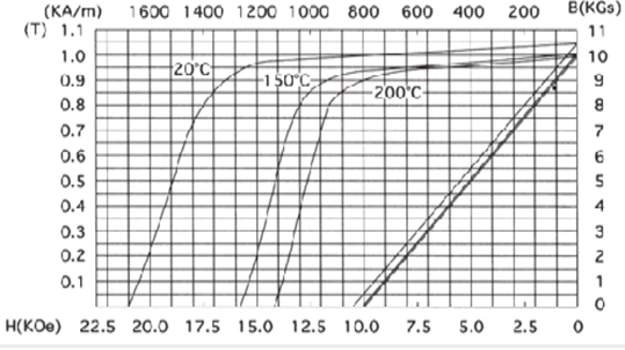
\includegraphics[width=0.7\textwidth]{figure/chapter3/demagnetization-SmCo5.png}
	\caption{喷嘴截面处冲砂液轴向流速对比图}
	\label{fig:demagnetization_SmCo5}
\end{figure}

\begin{figure}[htbp]
	\centering
	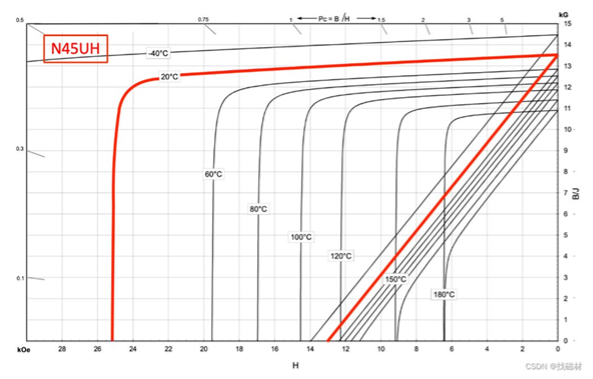
\includegraphics[width=0.7\textwidth]{figure/chapter3/demagnatization-N45UH.png}
	\caption{喷嘴截面处冲砂液轴向流速对比图}
	\label{fig:demagnatization_N45UH}
\end{figure}

\subsection{井筒清洁工具中磁铁布置研究}
在井筒清洁工具中实现磁铁的安装，重点需要考虑的是磁铁部件的安转和夹紧，便于工具的使用和维护，这种结构设计工作甚至需要借鉴设计者在井下工具结构设计方面的经验。在确定工具的基本结构后，需要重点考察磁铁的磁化以其他辅助结构的选材等问题。图为本项目设计的大容量强磁工具，其主要的功能单元包含上部强磁和下部强磁结构（如图2.3(b)、(c)）所示，两部分采用改了不同吸附结构，前者适于吸附小尺度铁质颗粒，后者适于吸附大尺度的铁质颗粒。上部强磁的磁铁放置于带窗的磁铁保护管中，增加与小尺度颗粒的接触面积，每个吸附单元包含两组磁铁，铁质碎屑将吸附于相邻吸附单元之间的空隙中。下部强磁采用开放式结构，磁铁的外圆面暴露于外，增强对大尺寸的铁质碎屑的捕捉能力。给定磁铁材料和吸附结构的情况下，工具的吸附能力主要依赖于磁铁的磁化方向和结构件的材料，下文将对此展开仿真研究。

\begin{figure}[htbp]
    \centering
    % 子图 (a)
    \subfloat[工具磁结构分布]{%
        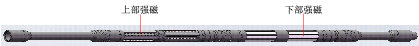
\includegraphics[width=0.9\linewidth]{figure/chapter3/magnetic-distribution-on-tool.png}%
        \label{fig:magnet_distribution_on_tool}%
    }
    \vspace{1em}
    % 子图 (b)
    \subfloat[上部强磁局部结构]{%
        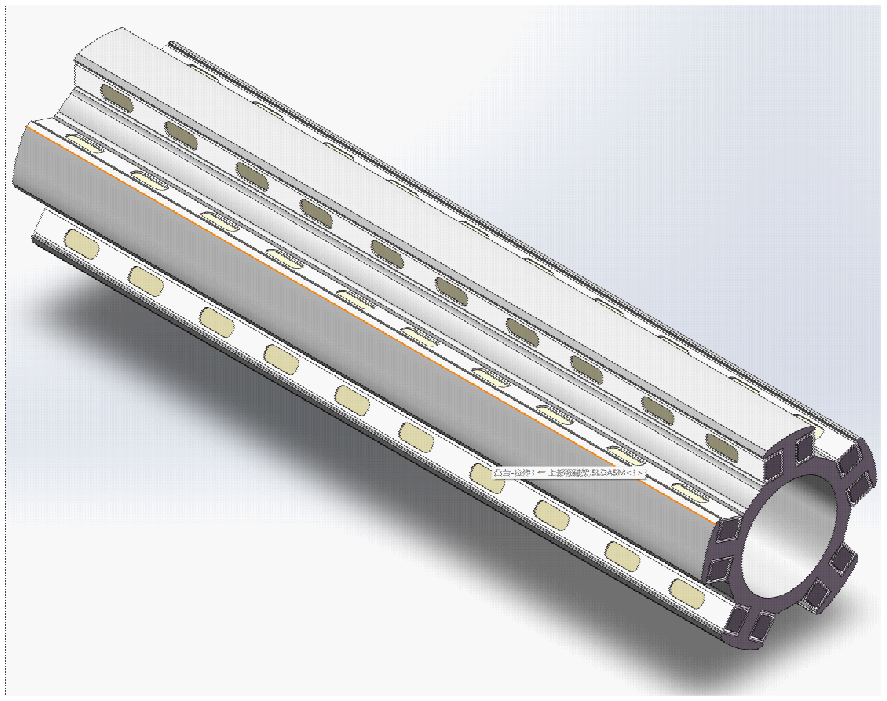
\includegraphics[width=0.4\linewidth]{figure/chapter3/structure-upper-magnetic-sub.png}%
        \label{fig:magnetic_tool_upper_sub}
    }
    \hfill
    % 子图 (c)
    \subfloat[上部强磁局部结构]{%
        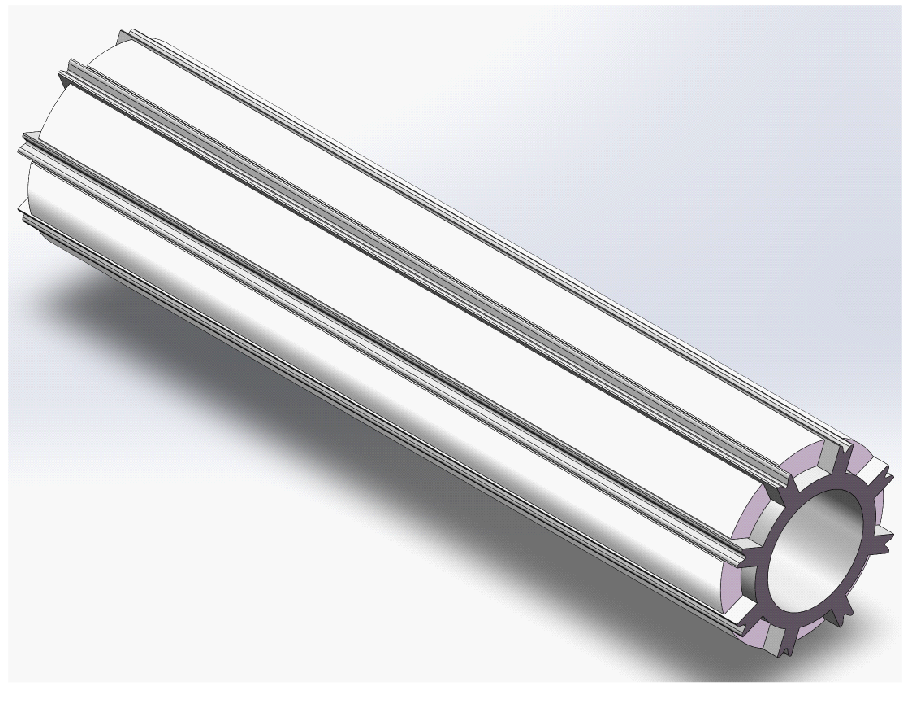
\includegraphics[width=0.4\linewidth]{figure/chapter3/structure-lowwer-magnetic-sub.png}%
        \label{fig:magnetic_tool_lowwer_sub}%
    }
        \caption{大容量强磁工具含磁结构示意图}
    \label{fig:structure_magnetic_tool}
\end{figure}

\subsubsection{强磁工具吸附力理论模型}
在井下环境中，强磁工具上永磁体对井筒内磁性废屑的吸附主要源于永磁体所产生的磁场与磁性材料的相互作用，磁性废屑在永磁体磁场中被磁化产生磁性并与永磁体产生相互作用力。此过程受磁场分布规律、磁场衰减特性、磁性材料磁化程度等多因素影响。
假设磁场均匀分布且磁性废屑与强磁工具上的永磁体直接接触时，其吸附力可利用麦克斯韦应力公式计算：
\begin{equation}
	F=\frac{B^2A}{2\mu_0}
\end{equation}
式中，$B$为永磁体与磁性物质接触表面的磁感应强度，$\mathrm{T}$；$A$为永磁体与磁性物质的接触面积，$\mathrm{m}^2$；$\mu_0$为真空磁导率常数，$\mu_0=4\pi×10^(-7) \mathrm{H/m}$。

当磁性铁屑与磁铁存在一定距离$d$时，吸附力需考虑磁场梯度的影响，这时永磁体对磁性碎屑的吸引力可表示为
\begin{equation}
	F=\frac{3\mu_0 m_1m_2}{4\pi d^4}
\end{equation}
式中，$m_1$ 、$m_2$分别为永磁体与磁性物质的磁矩，单位$\mathrm{A}\cdot \mathrm{m}^2$。

永磁体磁矩$m_1$的计算式为
\begin{equation}
	m_1=\frac{B_rV_1}{\mu_0}
\end{equation}
式中，$B_r$为永磁体剩磁，$\mathrm{T}$；$V_1$为永磁体体积，$\mathrm{m}^3$。

铁屑的磁矩$m_2$与所处的外磁感应场强度$B$有关，计算式为
	\begin{equation}
		m_2 = \frac{\gamma B V_2}{\mu_0}
	\end{equation}
式中，$\gamma$为磁性物质的磁化率，通常铁磁材料的$\gamma≫1$，量纲为1；$V_2$为磁性物质体积，$\mathrm{m}^3$。

综合以上两式，铁屑受到的磁力为
\begin{equation}
	F=\frac{3V_1V_2BB_r\gamma}{4\pi d^4}
\end{equation}

综上所述，在井下强磁工具吸附磁性废屑过程中，当永磁体体积参数确定时，体积越大、距离工具越近，周围磁场强度更高的磁性碎屑所受吸附力越大。在井下碎屑参数未知时，可选择高温度下剩磁高、体积大的磁体，以及保证工具外侧磁场强度大来产生足够大的吸附力。但采用解析方法精确计算碎屑受到的磁力难度较大：一方面，单个永磁体要受到其他永磁体及工具复杂结构的影响，永磁体的剩磁$B_r$难以确定；另一方面，磁性碎屑相互有之间会产生磁场的干扰，磁性碎屑堆积形成的碎屑床形状不规则，碎屑和磁铁之间的距离不能事先预测。于是，下文采用有限元的方法对工具空载（没有磁性碎屑存在）的条件下对工具周围磁场进行研究，作为一个表征工具碎屑吸附性能的间接指标，进而探索对工具性能产生影响的结构参数的影响。

\subsubsection{上部结构磁铁仿真模拟}

上部强磁结构为一三维结构，工具中的磁场应是一个复杂的三维空间磁场。但除端部外，其有效的功能单元是可看成是沿轴向均布的，于是，可考虑采用采用二维模型对所研究的问题进行简化。在ANSYS Maxwell软件中建立如图2.5所示的Maxwell 2D静磁场。永磁体材料选择井筒工作温度为$180\,^\circ \mathrm{C}$下的钐钴（SmCo5）材料，骨架材料选择4145牌号的钢材，永磁体保护套材料为304钢，各材料的属性列举于表\ref{tab:smco5_params}—表\ref{tab:304_properties_180c}中。


\begin{figure}[htbp]
	\centering
	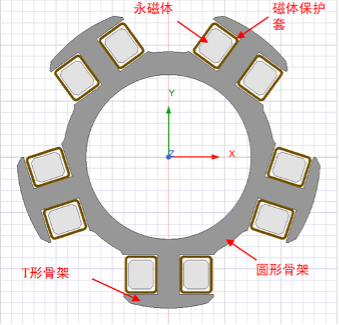
\includegraphics[width=0.5\textwidth]{figure/chapter3/magnet-configuration-upper-sub.png}
	\caption{强磁工具上部结构模型}
	\label{fig:magnet_configuration_upper_sub}
\end{figure}



\begin{table}[htbp]
    \centering
    \caption{$180\,^\circ\mathrm{C}$ SmCo5磁材性能参数表}
    \label{tab:smco5_params}
    \begin{tabularx}{.9\textwidth}{Xccc}
        \toprule
        参数 & 符号 & 数值 & 单位 \\
        \midrule
        相对磁导率 & $\mu$ & 1.09 & - \\
        剩磁 & $B_r$ & 0.8 & T \\
        电导率 & $\sigma$ & 1500000 & Siemens/s \\
        \midrule
        矫顽力 & $H_{cj}$ & $-15$ & kOe \\
        \bottomrule
    \end{tabularx}
\end{table}

\begin{table}[htbp]
    \centering
    \caption{$180\,^\circ\mathrm{C}$ 4145钢材性能参数表}
    \label{tab:steel_params}
    \begin{tabularx}{.9\textwidth}{Xccc}
        \toprule
        参数 & 符号 & 数值 & 单位 \\
        \midrule
        相对磁导率 & $\mu$ & 200 & --- \\
        电导率 & $\sigma$ & 4250000 & Siemens/s \\
        杨氏模量 & $E$ & 195 & GPa \\
        泊松比 & $\nu$ & 0.3 & --- \\
        \bottomrule
    \end{tabularx}
\end{table}

\begin{table}[htbp]
  \centering
  \caption{$180\,^\circ \mathrm{C}$下304不锈钢性能参数表}
  \label{tab:304_properties_180c}
  \begin{tabularx}{.9\textwidth}{Xccc}
    \toprule
    参数 & 符号 & 数值 & 单位 \\
    \midrule
    相对磁导率 & $\mu$ & 1 & --- \\
    电导率 & $\sigma$ & 1200000 & Siemens/s \\
    杨氏模量 & $E$ & 185 & GPa \\
    泊松比 & $v$ & 0.3 & --- \\
    \bottomrule
  \end{tabularx}
\end{table}


对于图\ref{fig:magnet_configuration_upper_sub}给定的磁铁、保护套和骨架结构，磁铁有图\ref{fig:two_magnetization_upper_sub}所示两种磁化方向，下文分别称为径向磁化和周向磁化。求解域设置为边长300mm的矩形，在其四条边上设置气球边界条件，网格划分，磁体与其保护套上最大网格尺寸0.5mm，上部结构骨架上最大网格尺寸2mm，求解步设置计算至收敛。在计算域中设置一个边长为200mm的矩形观测区域以观测仿真结果，以进行仿真结果后处理。

\begin{figure}[htbp]
    \centering
    % 子图 (a)
    \subfloat[径向磁化]{%
        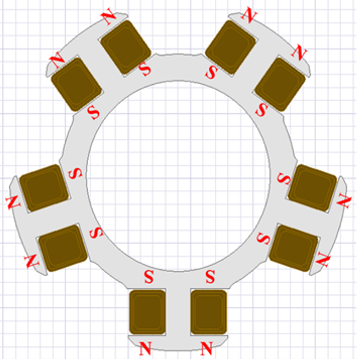
\includegraphics[width=0.35\linewidth]{figure/chapter3/radial-magnetization-in-upper-sub.png}%
        \label{fig:radial_magnetization_in_upper_sub}
    }
    %\hfill
    % 子图 (b)
    \subfloat[周向磁化]{%
        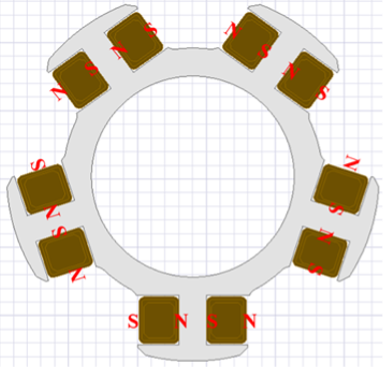
\includegraphics[width=0.35\linewidth]{figure/chapter3/circumferencial-magnetization-in-upper-sub.png}%
        \label{fig:circumferencial_magnetization_in_upper_sub}%
    }
        \caption{上部强磁两种磁化方向示意图}
    \label{fig:two_magnetization_upper_sub}
\end{figure}

\begin{figure}[htbp]
    \centering
    % 子图 (a)
    \subfloat[边界条件设置]{%
        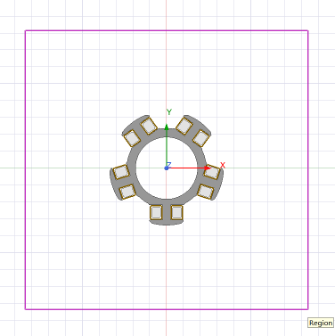
\includegraphics[width=0.35\linewidth]{figure/chapter3/boundary-condition-upper-sub.png}%
        \label{fig:boundary_condition_upper_sub}
    }
    \hfill
    % 子图 (b)
    \subfloat[计算域网格划分]{%
        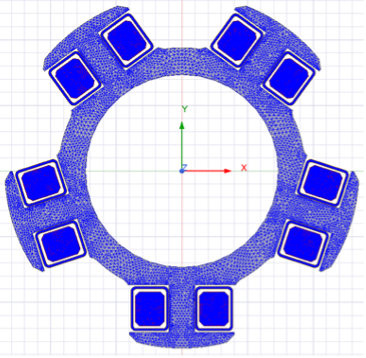
\includegraphics[width=0.35\linewidth]{figure/chapter3/mesh-upper-sub.png}%
        \label{fig:mesh_upper_sub}%
    }
        \caption{上部强磁磁场分析设置}
    \label{fig:computation_setup_upper_sub}
\end{figure}

(1) 径向充磁仿真结果及讨论

由于强磁工具在其使用工况下是通过其外侧磁场的作用吸附碎屑，因此在仿真结果中以强磁工具表面磁场强度为分析对象。

由观测面上的磁感应强度云图可知，最大磁感应强度$B=7.9T$，出现在永磁体安装T型骨架沟槽的顶部和底部；各永磁体表面的$B$值在$0.5$—$1.5T$范围内，但是受304不锈钢制的永磁体保护套影响，保护套外侧$B$值在$0.2$—$0.7T$范围内，T型骨架表面的$B$值在$0.6$—$1.4T$范围内，而圆形骨架的B值较低大部分在$0.5T$以下，从结果来看，304不锈钢制的永磁体保护套会使工具外侧的磁场强度变低。

\begin{figure}[htbp]
    \centering
    % 子图 (a)
    \subfloat[磁场矢量分布]{%
        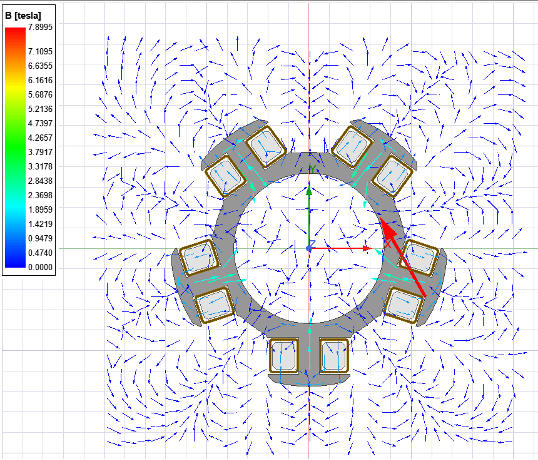
\includegraphics[width=0.45\linewidth]{figure/chapter3/magnetic-vector-distribution-upper-sub.png}%
        \label{fig:magnetic_vector_distribution_upper_sub}
    }
    %\hfill
    % 子图 (b)
    \subfloat[磁感应强度分布]{%
        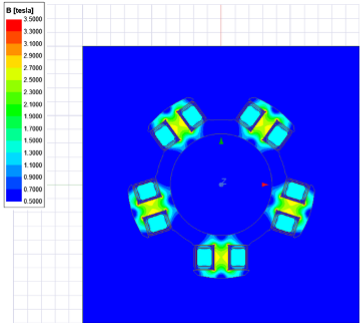
\includegraphics[width=0.45\linewidth]{figure/chapter3/contour-magnetic-field-upper-sub.png}%
        \label{fig:contour_magnetic_field_upper_sub}%
    }
        \caption{磁铁径向磁化时上部强磁组件磁场计算结果}
    \label{fig:field_result_in_upper_sub_radial_magnetization}
\end{figure}

(2) 周向充磁仿真结果及讨论

观察磁感应强度云图可知，观测面上最大磁感应强度$B=2.9T$，出现在T型骨架沟槽最顶部，永磁体内的$B$值在$0.6$—$1.3T$范围内，保护套上$B$值在$0.5$—$0.9T$范围内，T型骨架沟槽中的B值在$0.4$-$1.3T$范围内，而圆形骨架的$B$值在$0.3$—$0.8T$范围内。

\begin{figure}[htbp]
    \centering
    % 子图 (a)
    \subfloat[磁场矢量分布]{%
        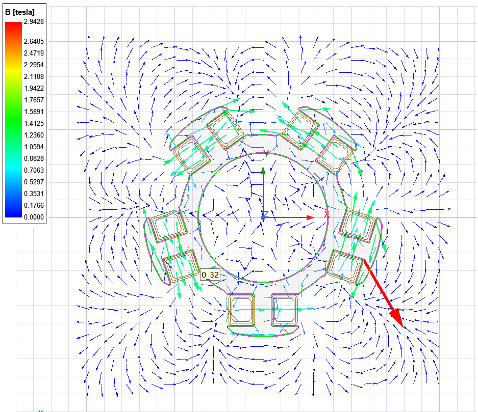
\includegraphics[width=0.45\linewidth]{figure/chapter3/magnetic-vector-distribution-upper-sub-circum-magnatization.png}%
        \label{fig:magnetic_vector_distribution_upper_sub_circum_magnatization.png}
    }
    \hfill
    % 子图 (b)
    \subfloat[磁感应强度分布]{%
        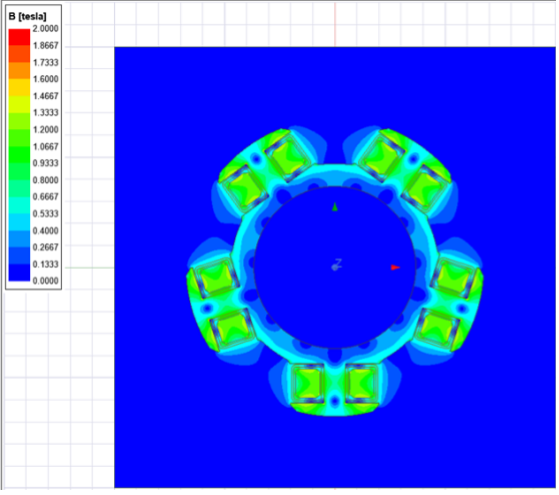
\includegraphics[width=0.45\linewidth]{figure/chapter3/contour-magnetic-field-upper-sub-circum-magnatization.png}%
        \label{fig:contour_magnetic_field_upper_sub_circum_magnatization}%
    }
        \caption{磁铁周向磁化时上部强磁组件磁场计算结果}
    \label{fig:field_result_in_upper_sub_radial_magnetization}
\end{figure}


上部结构中的两种充磁方式中，周向充磁磁场分布更加均匀，但最大磁感应强度值远小于径向充磁磁场，分析得出上部结构类型导致T型骨架和圆形骨架上的磁场分布存在差异，T型骨架上的场强大于圆形骨架上场强，不锈钢制的磁铁保护套会降低永磁体表面的磁场强度。分析两种充磁方式下各部表面磁感应强度表可知，周向充磁与径向充磁相比，永磁体及其保护套、T形骨架表面上的磁场强度差异较小，但圆形骨架表面磁场强度大于周向充磁时的磁场强度，周向充磁时磁场分布更加均匀，因此，对于上部结构宜选用周向充磁方式。

%这里差一个表2.5

\subsubsection{下部结构仿真模拟}

强磁工具下部结构为一对称结构，永磁体均匀排列在其骨架上，为方便仿真计算，将下部结构简化为二维模型求解，在ANSYS Maxwell软件中建立如图\ref{fig:magnet_configuration_lowwer_sub}所示的强磁工具下部结构仿真模型。永磁体材料选择井筒工作温度为180℃下的钐钴SmCo5材料，骨架材料选择4145牌号的钢材，各材料的属性见表\ref{tab:smco5_params}—表\ref{tab:304_properties_180c}。

\begin{figure}[htbp]
	\centering
	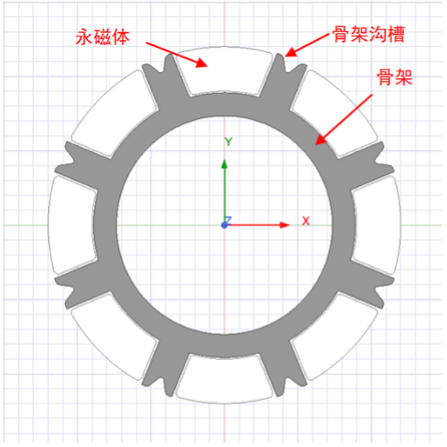
\includegraphics[width=0.5\textwidth]{figure/chapter3/magnet-configuration-lowwer-sub.png}
	\caption{强磁工具上部结构模型}
	\label{fig:magnet_configuration_lowwer_sub}
\end{figure}

对于强磁工具下部结构，磁铁有图2.6所示的同一径向磁化、交叉径向磁化、周向磁化三种磁化方向，其他仿真参数与上部结构仿真模型相同，如图\ref{fig:computation_setup_lowwer_sub}所示，对观测面上的仿真结果进行分析。三种磁化方式对应的磁场分布如图\ref{fig:field_result_in_lowwer_sub_3_magnetization}所示。


\begin{figure}[htbp]
    \centering
    % 子图 (a)
    \subfloat[同一径向磁化]{%
        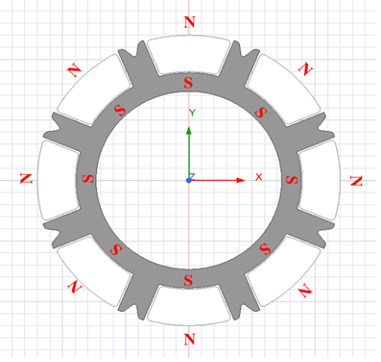
\includegraphics[width=0.4\linewidth]{figure/chapter3/lowwer-sub-magnetization-radial.png}%
        \label{fig:lowwe_sub_magnetization_radial}%
    }
    \vspace{1em}
    % 子图 (b)
    \subfloat[交叉径向磁化]{%
        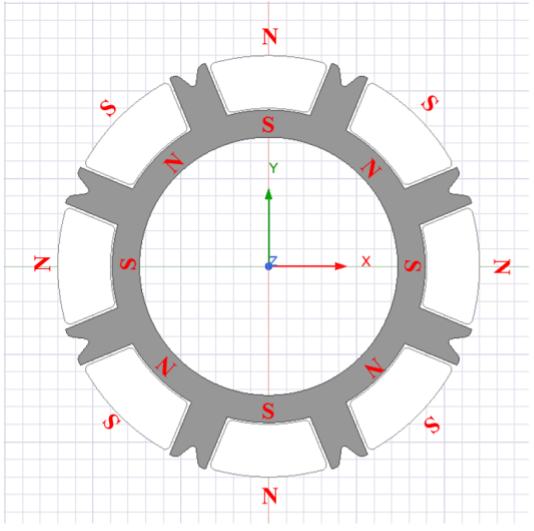
\includegraphics[width=0.4\linewidth]{figure/chapter3/lowwer-sub-cross-magnetization.png}%
        \label{fig:lowwer_sub_cross_magnetization}
    }
    \hfill
    % 子图 (c)
    \subfloat[周向磁化]{%
        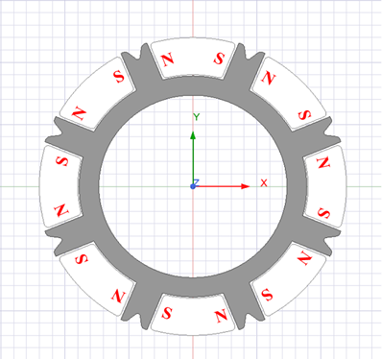
\includegraphics[width=0.4\linewidth]{figure/chapter3/lowwer-sub-circumferential-magnetization.png}%
        \label{fig:lowwer_sub_circumferential_magnetization}%
    }
        \caption{下部强磁磁化方向示意图}
    \label{fig:lowwer_sub_magnetization_3ways}
\end{figure}


\begin{figure}[htbp]
    \centering
    % 子图 (a)
    \subfloat[边界条件设置]{%
        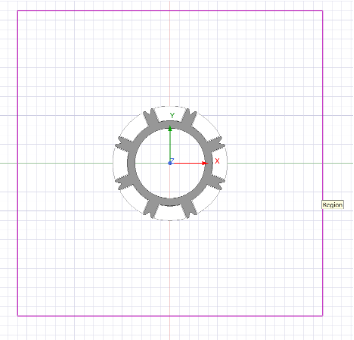
\includegraphics[width=0.4\linewidth]{figure/chapter3/boundary-condition-lowwer-sub.png}%
        \label{fig:boundary_condition_lowwer_sub}
    }
    %\hfill
    % 子图 (b)
    \subfloat[计算域网格划分]{%
        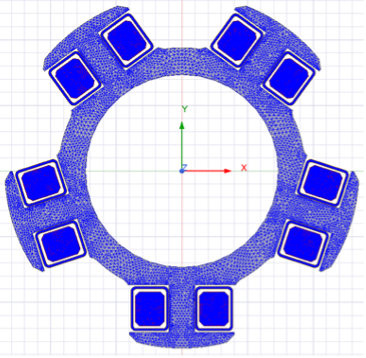
\includegraphics[width=0.4\linewidth]{figure/chapter3/mesh-upper-sub.png}%
        \label{fig:mesh_lowwer_sub}%
    }
        \caption{下部强磁磁场分析设置}
    \label{fig:computation_setup_lowwer_sub}
\end{figure}



\begin{figure}[htbp]
    \centering
    % 子图 (a)
    \subfloat[磁场矢量分布]{%
        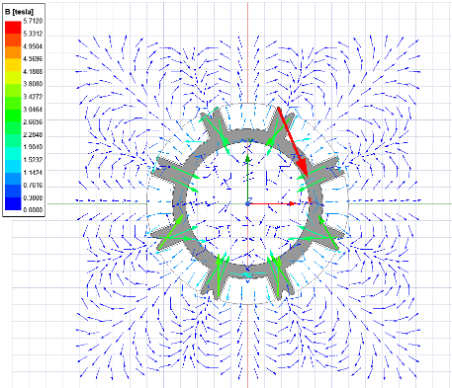
\includegraphics[width=0.45\linewidth]{figure/chapter3/magnetic-vector-distribution-lowwer-sub-radial.png}%
        \label{fig:magnetic_vector_distribution_lowwer_sub_radial}
    }
    %\hfill
    % 子图 (b)
    \subfloat[磁感应强度分布]{%
        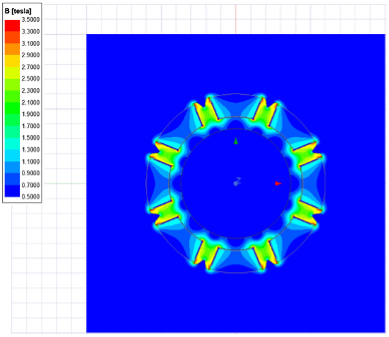
\includegraphics[width=0.45\linewidth]{figure/chapter3/contour-magnetic-field-lowwer-sub-radial.png}%
        \label{fig:contour_magnetic_field_lowwer_sub_radial}%
    }
    \vspace{1em}
     % 子图 (c)
    \subfloat[磁场矢量分布]{%
        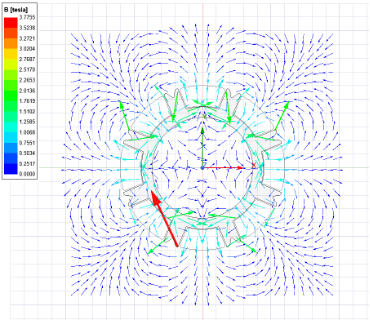
\includegraphics[width=0.45\linewidth]{figure/chapter3/magnetic-vector-distribution-lowwer-sub-cross.png}%
        \label{fig:magnetic_vector_distribution_lowwer_sub_cross}
    }
   % \hfill
    % 子图 (d)
    \subfloat[磁感应强度分布]{%
        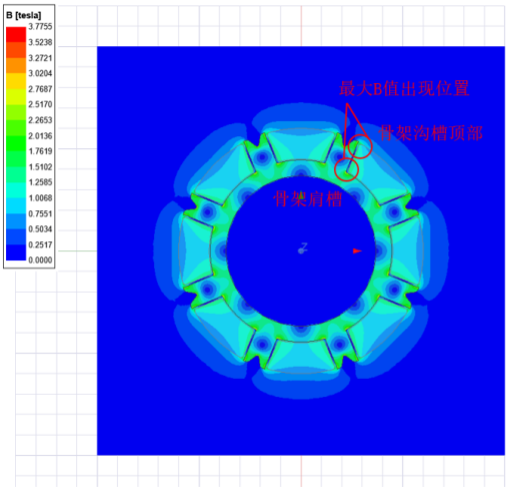
\includegraphics[width=0.45\linewidth]{figure/chapter3/contour-magnetic-field-lowwer-sub-cross.png}%
        \label{fig:contour_magnetic_field_lowwer_sub_cross}%
    }
    \vspace{1em}
     % 子图 (e)
    \subfloat[磁场矢量分布]{%
        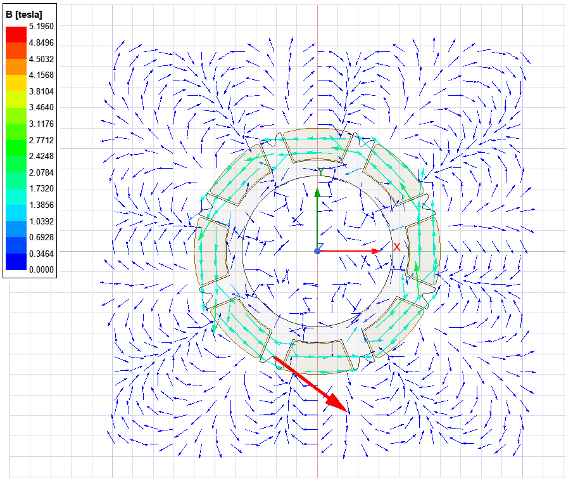
\includegraphics[width=0.45\linewidth]{figure/chapter3/magnetic-vector-distribution-lowwer-sub-circumferential.png}%
        \label{fig:magnetic_vector_distribution_upper_sub_circumferential}
    }
   % \hfill
    % 子图 (f)
    \subfloat[磁感应强度分布]{%
        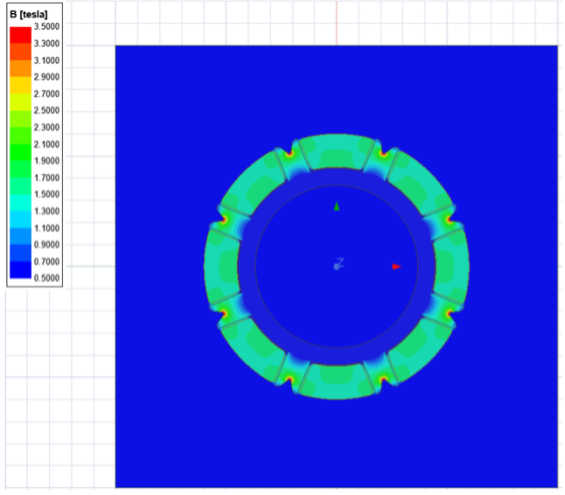
\includegraphics[width=0.45\linewidth]{figure/chapter3/contour-magnetic-field-lowwer-sub-circumferential.png}%
        \label{fig:contour_magnetic_field_upper_sub_circumferential}%
    }


        \caption{磁铁采用不同磁化方式时下部强磁组件磁场计算结果}
    \label{fig:field_result_in_lowwer_sub_3_magnetization}
\end{figure}




(1) 同一径向充磁仿真结果及讨论

由观测面上的磁感应强度云图可知，磁感应强度成对称分布，最大磁感应强度B=5.7 T，出现在永磁体安装骨架的肩槽和骨架沟槽顶部，各永磁体表面的B值在0.5—1.5T范围内，骨架沟槽表面的B值在骨架最凹处最小沿沟槽向两侧增大其数值在0.5—3.5T范围内。

(2) 交叉径向充磁仿真结果及讨论

由观测面上的磁感应强度云图可知，磁感应强度称对称分布，最大磁感应强度B=3.8 T，出现在永磁体安装骨架的肩槽和骨架沟槽顶部，各永磁体表面的B值在0.7—1.5T范围内，骨架沟槽表面的B值在1.2—3.5T范围内。

(3) 周向充磁仿真结果及讨论

由观测面上的磁感应强度云图可知，云图上最大磁感应强度B=5.2T出现在骨架沟槽最凹点处，各永磁体上的B值在1.3—1.7T范围内，骨架沟槽表面最凹点B值最大沿沟槽向两侧减小，其数值在0.7-3.5T范围内。


由基于充磁方式的下部强磁工具仿真结果总结于表\ref{tab:magnetic_intensity}，由此可得出，永磁体表面的磁感应强度周向充磁时略强于径向充磁时，分析骨架沟槽的表面的磁感应强度可知，同一径向充磁和周向充磁时，骨架沟槽上的磁感应强度梯度大，交叉径向充磁时骨架沟槽表面的磁感应强度分布更均匀。同一径向充磁和周向充磁时，磁感线会富集到骨架沟槽内造成骨架沟槽内的磁感应强度大，而工具外侧的磁感应强度小。因此，下部结构宜选择交叉径向充磁方式。

\begin{table}[htbp]
    \centering
    \caption{下部结构各部表面磁感应强度数据}
    \label{tab:magnetic_intensity}
    \begin{tabularx}{.9\textwidth}{Xccc} % 第一列左对齐(l)，后三列居中(c)
        \toprule
        % 第一行：左侧标题 + 右侧跨3列的标题
        强磁工具结构 & \multicolumn{3}{c}{下部结构} \\
        \midrule
        % 第二行：具体的充磁类型分类
        充磁类型 & 同向径向充磁 & 交叉径向充磁 & 周向充磁 \\
        \midrule
        % 第三行：数据
        永磁体表面 & 0.5---1.5T & 0.7---1.5T & 1.3---1.7T \\
        % 第四行：数据
        骨架沟槽表面 & 0.5---3.5T & 1.2---3.5T & 0.7---3.5T \\
        \bottomrule
    \end{tabularx}
\end{table}

\subsection{两种结构对强磁工具最大磁性分布的影响}

本节依据上节两种强磁工具结构的仿真结果，通过数据对比分析两种结构对强磁工具磁性分布的影响。强磁工具各部表面磁感应强度数值由磁场探针测得，测量数据见表\ref{tab:strong_magnet_data}。



\begin{table}[htbp]
    \centering
    \caption{强磁工具各部表面磁感应强度数据表}
    \label{tab:strong_magnet_data}
    % 设置列格式：第一列左对齐，其余居中。p{}用于控制长文本换行
    \begin{tabular}{lcccccc}
        \toprule
        % 第一行表头：上部结构(跨2列)，下部结构(跨3列)
        强磁工具结构 & \multicolumn{2}{c}{上部结构} & \multicolumn{4}{c}{下部结构} \\
        \cmidrule(r){2-3} \cmidrule(l){4-7} % 子表头下方的横线，r/l控制留白
        % 第二行表头：具体的充磁类型
        充磁类型 & 径向充磁 & 周向充磁 & \shortstack{同向径向\\充磁} & \shortstack{交叉径向\\充磁} & \multicolumn{2}{c}{周向充磁} \\
        \midrule
        % 数据行 1
        永磁体表面 & 0.5---1.5T & 0.6---1.3T & 0.5---1.5T & 0.7---1.5T & \multicolumn{2}{c}{1.3---1.7T} \\
        % 数据行 2 (包含合并行 "骨架沟槽表面")
        T型骨架表面 & 0.6---1.4T & 0.4---1.3T & \multirow{2}{*}{\shortstack{骨架沟槽\\表面}} & 0.5---3.5T & 1.2---3.5T & 0.7---3.5T \\
        % 数据行 3
        圆形骨架表面 & 0---0.3T & 0.3---0.8T & & - & - & - \\
        % 数据行 4
        保护套表面 & 0.2---0.7T & 0.5---0.9T & - & - & - & - \\
        \bottomrule
    \end{tabular}
\end{table}

由强磁工具的上、下部结构在不同充磁方向下的各部位表面磁场数据得出，对于上部结构，由于其结构影响T型骨架和圆形骨架上的磁场分布差异较大，T型骨架上场强大于圆形骨架上的场强，且不锈钢保护套会造成永磁体表面磁场衰减，改变永磁体充磁方向后磁场分布仍呈现此情况；对于下部结构，不同的充磁方向对其表面磁场分布影响很大，永磁体采用交叉径向充磁时，工具永磁体和骨架的表面磁场分布均匀。综上所述，采用交叉径向充磁的下部强磁工具结构的表面磁场分布均匀，易于强磁工具在井筒内的大面积吸附工作。


\subsection{强磁工具骨架材料对最大磁性分布的影响}

利用2.2.4小节中的下部工具结构仿真模型数据，保持其他仿真参数不变，在永磁体交叉径向充磁的工况下，将强磁工具骨架材料设置为不导磁的铝材，铝材参数如表\ref{tab:aluminum_params}所示，观察仿真结果中工具表面磁场分布。下部结构交叉径向充磁时，铝制骨架与4145钢制骨架模型的仿真结果进行对比分析图\ref{fig:mag_field_frame_material}。

\begin{table}[htbp]
    \centering
    \caption{180$^\circ$C下铝材参数表}
    \label{tab:aluminum_params}
    \begin{tabularx}{.9\textwidth}{Xccc}
        \toprule
        参数 & 符号 & 数值 & 单位 \\
        \midrule
        相对磁导率 & $\mu$ & 1.00021 & --- \\
        电导率 & $\sigma$ & 38000000 & Siemens/s \\
        杨氏模量 & $E$ & 69 & GPa \\
        泊松比 & $\nu$ & 0.31 & --- \\
        \bottomrule
    \end{tabularx}
\end{table}

\begin{figure}[htbp]
    \centering
    % 子图 (a)
    \subfloat[4145钢制骨架]{%
        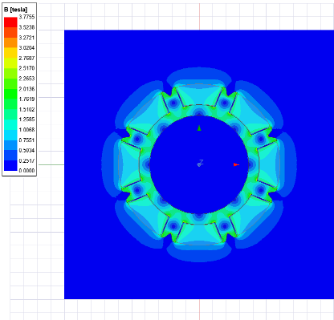
\includegraphics[width=0.4\linewidth]{figure/chapter3/mag-field-distribution-4145-steel-frame.png}%
        \label{fig:mag_field_distribution_4145_steel_frame}
    }
    \hfill
    % 子图 (b)
    \subfloat[铝制骨架]{%
        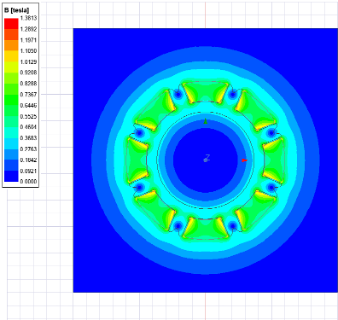
\includegraphics[width=0.4\linewidth]{figure/chapter3/mag-field-distribution-aliminium-frame.png}%
        \label{fig:mag_field_distribution_aliminium_frame}%
    }
        \caption{骨架材料对磁场分布的影响}
    \label{fig:mag_field_frame_material}
\end{figure}

表\ref{tab:aluminum_vs_4145_steel}为下部强磁工具结构交叉径向充磁模型的4145钢制骨架和铝制骨架仿真结果对比。由铝制骨架仿真结果得出，铝制骨架导致工具磁场中的最大场强降低，铝制骨架沟槽内的磁场强度低于4145钢制骨架沟槽内的磁场强度，分析得出骨架材料宜选用导磁效果好，可磁化程度高的金属合金材料，以起到聚集磁感线增大磁通的效果。


\begin{table}[htbp]
    \centering
    \caption{铝制骨架与4145钢制骨架工具表面磁场数据对比}
    \label{tab:aluminum_vs_4145_steel}
    \begin{tabularx}{.9\textwidth}{Xcc}
        \toprule
        强磁工具结构 & \multicolumn{2}{c}{下部结构} \\
        \cmidrule(r){2-3}
        充磁类型 & \multicolumn{2}{c}{周向充磁} \\
        \cmidrule(r){2-3}
        骨架材料 & 4145 钢制 & 铝制 \\
        \midrule
        永磁体表面 & 0.7---1.5T & 0.3---0.7T \\
        骨架沟槽表面 & 1.2---3.5T & 0.2---0.4T \\
        \bottomrule
    \end{tabularx}
\end{table}

\subsection{永磁材料的退磁影响因素}

永磁体的退磁是影响其长期稳定性和应用可靠性的关键问题，退磁由多种因素引起。

（1）居里温度

居里温度是磁性材料在铁磁性物质/亚铁磁性物质和顺磁性物质之间改变的温度。温度超过居里温度，磁体内部分子剧烈运动并出现不可逆的退磁情况，磁体退磁后可再次被充磁，但磁力会大幅下降，仅能达到原来的50\%左右。

（2）工作温度

在工作温度内温度升高磁力会下降，但是不超过居里温度的情况下，降温后磁力大部分会恢复，工作温度范围内发生可逆性退磁。

（3）外部磁场

外部强反向磁场（如电机电枢反应、短路电流）可能超过磁体的矫顽力，导致磁体部分或完全退磁。

（4）时间因素

随着时间的延长磁体内部微观结构（如晶粒边界、杂质相）随时间缓慢变化，导致剩磁轻微衰减，通常每年衰减小于1\%。

（5）机械冲击

机械应力可能破坏磁体内部的磁畴排列，尤其是脆性材料（如钕铁硼），避免直接敲击或跌落磁体。在复杂振动环境中增加缓冲结构（如橡胶垫）。

（6）化学侵蚀

在高温、高湿的酸碱环境下，钕铁硼磁体因含钕、铁易氧化（生锈），导致磁通量下降甚至断裂。在不稳定的化学环境下对磁体进行表面涂层（如镍、锌、环氧树脂、电镀层）或密封封装以隔绝环境影响。

具体到井筒清洁工具设计，具体到井筒清洁工具的设计，选择的钐钴磁铁耐温达到了450—550$^\circ$C，磁材的居里温度为750—850$^\circ$C，远超工具的设计温度指标150$^\circ$C，可保证磁铁不会因温度因素而退磁，在重复使用过程中，可保证磁材都是可逆退磁。井筒中不存在可能使磁铁退磁强外部磁场，磁铁在工作过程中的退磁效应可忽略。在工具长时间存储时，可考虑采用铁磁质材料制作的磁路附件使得磁材的磁路闭合，减少磁材磁性的衰减。在机械结构设计上，磁铁外设计了不锈钢制作的保护套，以减少清洁工具在运输和使用过程中产生的冲击直接作用于磁铁本身，减少机械冲击。在磁铁在制造过程中表面采用镀镍工艺，易蚀性磁材本体和腐蚀性的环境隔离开来，磁铁在安装过程中设置了安装规范，减少磁材表面划伤，严禁损伤磁材下井。

\subsubsection{强磁工具操作方式}

（1）使用方法

根据井眼尺寸选择合适的强磁吸附工具。强磁工具通过钻柱送入井底完成吸附打捞作业，如情况允许也可以通过钢丝绳送入井底。

（2）操作方法

该工具可以与ZKG模块化多合一套管清洁工具一同使用（推荐），也可以在刮完井之后使用。将强磁吸附工具放在预先放好木板的转盘上（防止强磁吸附工具与转盘发生吸附），并接于钻柱底部，然后提起，取掉木板，准备下井。将DQC大容量强磁吸附工具下到井下离通井位置3-5m处，开泵循环。将DQC大容量强磁吸附工具在该位置上下活动。保持循环，平稳地上提钻柱。起钻时要求平稳、低速、严禁剧烈震动与撞击，以保护强磁部件。

\subsubsection{强磁工具维护与保养}

DQC大容量强磁吸附工具每次使用后，应放在没有铁屑和杂物区域内的木板或橡胶板上，清除干净吸附在强磁工具表面的金属颗粒和铁屑粉末，然后用清水清洗各零件。工具在井下工作多次后，或在恶劣条件下工作后，应进行维护修理，将其全部拆开、检查、重新装配。



本节首先调研了钕铁硼、铝镍钴、钐钴等永磁材料的工作参数及退磁曲线，确定了钐钴材料为井下强磁工具上的永磁体材料并分析了永磁体退磁影响因素；其次，利用ANSYS Maxwell软件构建了上部强磁结构和下部强磁结构的仿真模型，通过改变工具中永磁体充磁方式及骨架材料，探究其最大磁性分布规律；在基于充磁方向的磁体布置研究中得出，上部结构宜采用径向充磁方式，下部结构宜采用周向充磁方式来达到磁场分布均匀且保证最大磁性的目的；在基于骨架材料对最大磁性分布的影响研究中得出，骨架材料为导磁效果好的金属材料时，能聚集磁感线增大磁通，起到增加工具磁性的作用。

































































